\setcounter{section}{2}
\section{Các khái niệm mở đầu}
\subsection{Tóm tắt lí thuyết}
% \begin{boxtb}
	\subsubsection{Khái niệm vectơ}
	\begin{dn}{}
		Vectơ là một đoạn thẳng có hướng.
	\end{dn}
    Vectơ có điểm đầu là $A$, điểm cuối là $B$ được kí hiệu là $\vec{AB}$, đọc là \lq\lq vectơ $AB$\rq\rq.
    \immini{
       Để vẽ vectơ $\vec{AB}$ ta vẽ đoạn thẳng $AB$ và đánh dấu mũi tên ở đầu mút $B$ (Hình 1).\\
       Đối với vectơ $AB$, ta gọi
       \begin{itemize}
       	\item Đường thẳng $d$ đi qua hai điểm $A$ và $B$ là giá của vectơ $AB$ (Hình 2).
       	\item Độ dài đoạn thẳng $AB$ là độ dài của vectơ $AB$, kí hiệu là $\left| \vec{AB}\right|$.
       \end{itemize}
}{
       \begin{tikzpicture}[scale=1, line join=round, line cap=round,font=\footnotesize,>=stealth]
       	\draw[->,line width= 1pt] (0,0)node[above]{$A$}--(4,0) node[above]{$B$};
       	\draw[->] (0,0)node[below]{Điểm đầu}--(4,0) node[below]{Điểm cuối};
       	\draw (2,-0.5) node[below]{Hình 1};
       	\fill[color=red] (0,0) circle(2pt) (4.05,0) circle(2pt);
       	\begin{scope}[shift={(0,-2)}]
       		\draw[-] (-0.3,0)--(4.8,0)node[above]{$d$};
       		\draw[->,line width= 1pt] (0,0)node[above]{$A$}--(4,0) node[above]{$B$};
       		\draw (2,0) node[below]{Hình 2};
       		\fill[color=red] (0,0) circle(2pt) (4.05,0) circle(2pt);
       	\end{scope}
       \end{tikzpicture}
}
%     \begin{vd}
%     	\immini{
%     	Cho hai điểm phân biệt $H$, $K$ như hình bên. Viết hai vectơ mà điểm đầu và điểm cuối là $H$ hoặc $K$.
%     }{
%         \begin{tikzpicture}[scale=1, line join=round, line cap=round,font=\footnotesize,>=stealth]
%         	\draw[step=1cm,gray!50,very thin] (0.5,0.5) grid (3.5,2.5);
%         	\draw (1,1)node[below]{$H$} (3,2)node[below]{$K$};
%         	\fill[color=red] (1,1) circle(2pt) (3,2) circle(2pt);
%         \end{tikzpicture}
% }
%     	\loigiai{
%     	Hai vectơ thỏa mãn yêu cầu đề bài là $\vec{HK}$ và $\vec{KH}$.
%     }
%     \end{vd}
%     \begin{vd}
%     	\immini{
%     	Tính độ dài của các vectơ $\vec{AB}$, $\vec{CD}$ và $\vec{MN}$ ở Hình 3, biết rằng độ dài cạnh của ô vuông bằng $1$ cm.
%     }{
%         \begin{tikzpicture}[scale=0.6, line join=round, line cap=round,font=\footnotesize,>=stealth]
%         	\draw[step=1cm,gray!50,very thin] (0,0) grid (12,7);
%         	\draw[->,line width= 1pt] (1,1)node[below left]{$M$}--(4,4) node[above right]{$N$};
%         	\draw[->,line width= 1pt] (2,6)node[above]{$A$}--(6,6) node[above]{$B$};
%         	\draw[<-,line width= 1pt] (7,4.5)node[below]{$D$}--(11,4.5) node[below]{$C$};
%         	\fill[color=red] (1,1) circle(2pt) (4.05,4.05) circle(2pt) (6.95,4.5) circle(2pt) (11,4.5) circle(2pt) (2,6) circle(2pt) (6.05,6) circle(2pt);
%         	\draw (6,0) node[below]{Hình 3};
%         \end{tikzpicture}
% }
%     	\loigiai{
%     	\begin{align*}
%     		&\left|\vec{AB} \right| = AB = 4 \textrm{ cm}, \left|\vec{CD} \right| = CD = 4 \textrm{ cm},\\
%     		&\left|\vec{MN} \right| = MN = \sqrt{3^2 + 4^2} = 5 \textrm{ cm.}   
%     	\end{align*}
%     }
%     \end{vd}
    \subsubsection{Hai vectơ cùng phương, cùng hướng, bằng nhau}
%     \begin{dn}{}
%     	Hai vectơ được gọi là cùng phương nếu giá của chúng song song hoặc trùng nhau.
%     \end{dn}
%     \textbf{Nhận xét:} Nếu hai vectơ cùng phương thì hoặc chúng cùng hướng hoặc chúng ngược hướng.
%     \begin{vd}
%     	\immini{
%     	Trong Hình 4, tìm vectơ cùng hướng với vectơ $\vec{AB}$; ngược hướng với vectơ $\vec{AB}$.
%     }{
%         \begin{tikzpicture}[scale=0.6, line join=round, line cap=round,font=\footnotesize,>=stealth]
%         	\draw[step=1cm,gray!50,very thin] (0,0) grid (9,3.5);
%         	\draw[->,line width= 1pt] (1,1)node[below]{$A$}--(4,1) node[below]{$B$};
%         	\draw[->,line width= 1pt] (6,1)node[below]{$C$}--(8,1) node[below]{$D$};
%         	\draw[<-,line width= 1pt] (3,2)node[above]{$N$}--(6,2) node[above]{$M$};
%         	\fill[color=red] (1,1) circle(2pt) (4.05,1) circle(2pt) (6,1) circle(2pt) (8.05,1) circle(2pt) (2.95,2) circle(2pt) (6,2) circle(2pt);
%         	\draw (4.5,0) node[below]{Hình 4};
%         \end{tikzpicture}
% }
%     	\loigiai{
%     	vectơ $\vec{CD}$ cùng hướng với vectơ $\vec{AB}$, vectơ $\vec{MN}$ ngược hướng với vectơ $\vec{AB}$.
%     }
%     \end{vd}
    \begin{dn}{}
    	Hai vectơ $\vec{AB}$, $\vec{CD}$ bằng nhau nếu chúng cùng hướng và cùng độ dài, kí hiệu: $\vec{AB} = \vec{CD}$.
    \end{dn}
    \immini{
    Khi không cần chỉ rõ điểm đầu và điểm cuối của vectơ, vectơ còn được kí hiệu là $\vec{a}$, $\vec{b}$, $\vec{u}$, $\vec{v}$, \dots (Hình 5). Độ dài của vectơ $\vec{a}$ được kí hiệu là $\left| \vec{a} \right|$.
}{
    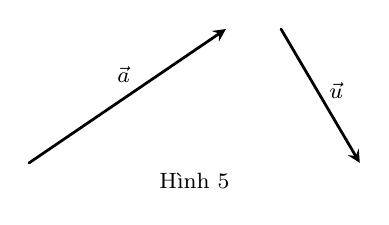
\begin{tikzpicture}[scale=1, line join=round, line cap=round,font=\footnotesize,>=stealth]
    	\draw[->,line width= 1pt] (0,0)--(2.5,1.7);
    	\draw[->,line width= 1pt] (3.2,1.7)--(4.2,0);
    	\draw (1.2,0.9)node[above]{$\vec{a}$} (3.9,0.7)node[above]{$\vec{u}$};
    	\draw (2.1,0) node[below]{Hình 5};
    \end{tikzpicture}
}
    \textbf{Nhận xét}
    \begin{itemize}
    	\item Hai vectơ $\vec{a}$, $\vec{b}$ bằng nhau nếu chúng cùng hướng và cùng độ dài, kí hiệu là $\vec{a} = \vec{b}$.
    	\item Khi cho trước vectơ $\vec{a}$ và điểm $O$, thì ta luôn tìm được một điểm $A$ duy nhất sao cho $\vec{OA} = \vec{a}$.
    \end{itemize}
%     \begin{vd}
%     	\immini{
%     	Cho hình bình hành $ABCD$ (Hình 6).
%     	\begin{enumerate}
%     		\item vectơ nào bằng vectơ $\vec{AB}$?
%     		\item vectơ nào bằng vectơ $\vec{AD}$?
%     	\end{enumerate}
%     }{
%         \begin{tikzpicture}[scale=0.8, line join=round, line cap=round,font=\footnotesize,>=stealth]
%         	\draw[step=1cm,gray!50,very thin] (0.2,0.3) grid (5.5,3.8);
%         	\draw[-,line width= 1pt] (2,3)node[above left]{$A$}--(5,3) node[above right]{$B$}--(4,1)node[below right]{$C$}--(1,1)node[below left]{$D$}--(2,3);
%         	\draw (2.7,0.3) node[below]{Hình 6};
%         \end{tikzpicture}
% }
%         \loigiai{
%         \begin{enumerate}
%         	\item Vì $\vec{AB}$, $\vec{DC}$ cùng hướng và $AB = DC$ nên $\vec{DC} = \vec{AB}$.
%         	\item Vì $\vec{AD}$, $\vec{BC}$ cùng hướng và $AD = BC$ nên $\vec{AD} = \vec{BC}$.
%         \end{enumerate}
%     }
%     \end{vd}
    \subsubsection{Vectơ không}
    \begin{dn}{}
    	vectơ không là vectơ có điểm đầu và điểm cuối trùng nhau, kí hiệu là $\vec{0}$.
    \end{dn}
    Với các điểm bất kì $A$, $B$, $C$ ta có $\vec{0} = \vec{AA} =\vec{BB} = \vec{CC}$.\\
    vectơ $\vec{AA}$ nằm trên mọi đường thẳng đi qua $A$. Ta quy ước $\vec{0}$ (vectơ không) cùng phương và cùng hướng với mọi vectơ; hơn nữa $\left| \vec{0} \right| = 0$.\\
    \textbf{Nhận xét:} Hai điểm $A$, $B$ trùng nhau khi và chỉ khi $\vec{AB} = \vec{0}$.
% \end{boxtb}


\subsection{Các dạng toán}

\begin{dang}{Xác định một vectơ, độ dài vectơ}
	\begin{itemize}
		\item vectơ là một đoạn thẳng có hướng, nghĩa là, trong hai điểm mút của đoạn thẳng, đã chỉ rõ điểm đầu, điểm cuối.
		\item Độ dài của vectơ là khoảng cách giữa điểm đầu và điểm cuối của vectơ đó.
	\end{itemize}
\end{dang}	

\viduminhhoa
\begin{vd}%[Vương Quyền]
	Cho tứ giác $ABCD$. Hãy chỉ ra các vectơ khác vectơ không có điểm đầu và điểm cuối là các đỉnh của tứ giác.
	\loigiai{
		\immini{
			Từ hai điểm phân biệt của tứ giác ta xác định được hai vectơ khác vectơ không,  chẳng hạn từ hai điểm $A$, $B$ ta xác định được hai vectơ khác vectơ không là $\overrightarrow{AB}$ và $\overrightarrow{BA}$.\\
			Suy ra tứ giác $ABCD$ có $12$ vectơ khác vectơ không là $\overrightarrow{AB}$, $\overrightarrow{BA}$, $\overrightarrow{AC}$, $\overrightarrow{CA}$, $\overrightarrow{AD}$, $\overrightarrow{DA}$, $\overrightarrow{BC}$, $\overrightarrow{CB}$, $\overrightarrow{BD}$, $\overrightarrow{DB}$, $\overrightarrow{BD}$, $\overrightarrow{DB}$.
		}{
			\begin{tikzpicture}[scale=0.8, font=\footnotesize, line join=round, line cap=round, >=stealth]
				\path
				(0,0)coordinate(A)
				(4,0)coordinate(B)
				(5,4)coordinate(C)
				(0,3)coordinate(D)
				;
				\draw(A)--(B)--(C)--(D)--(A);
				\foreach \x/\i in {A/180,B/0,C/10,D/160}{\path ($(\x)+(\i:3mm)$) node{$\x$};}
				\foreach \x in {A,B,C,D}{\draw[fill=black] (\x) circle (1pt);}
			\end{tikzpicture}
		}
	}
\end{vd}

\begin{vd}%[Vương Quyền]
	Cho hình vuông $ABCD$ với cạnh có độ dài bằng $1$. Tính độ dài các vectơ $\overrightarrow{AB}$, $\overrightarrow{BD}$, $\overrightarrow{DB}$.
	\loigiai{
		\immini{
			Vì cạnh của hình vuông $ABCD$ có độ dài bằng $1$ nên $|\overrightarrow{AB}|=1$ và đường chéo của hình vuông có độ dài bằng $\sqrt{2}$.\\
			Suy ra $|\overrightarrow{BD}|=|\overrightarrow{DB}|=BD=\sqrt{2}$.
		}{
			\begin{tikzpicture}[scale=0.8, font=\footnotesize, line join=round, line cap=round, >=stealth]
				\path
				(0,0)coordinate(A)
				(4,0)coordinate(B)
				(4,4)coordinate(C)
				(0,4)coordinate(D)
				;
				\draw(A)--(B)--(C)--(D)--(A);
				\foreach \x/\i in {A/180,B/0,C/10,D/160}{\path ($(\x)+(\i:3mm)$) node{$\x$};}
				\foreach \x in {A,B,C,D}{\draw[fill=black] (\x) circle (1pt);}
			\end{tikzpicture}
		}
	}
\end{vd}

\begin{vd}%[Vương Quyền]
	Cho tam giác đều $ABC$ có cạnh bằng $a$. Gọi $M$ là trung điểm của $BC$ tính độ dài vectơ $\overrightarrow{AM}$.
	\loigiai{
		\immini{
			Vì $ABC$ là tam giác đều nên $AM=\dfrac{a\sqrt{3}}{2}\Rightarrow|\overrightarrow{AM}|=AM=\dfrac{a\sqrt{3}}{2}$.	
		}{
			\begin{tikzpicture}[scale=1, font=\footnotesize, line join=round, line cap=round, >=stealth]
				\path
				(0:0)coordinate(A)
				(-60:3)coordinate(B)
				(-120:3)coordinate(C)
				($(B)!0.5!(C)$)coordinate(M)
				;
				\draw(A)--(B)--(C)--(A)--(M);
				\foreach \x/\i in {A/90,B/-90,C/-90,M/-90}{\path ($(\x)+(\i:3mm)$) node{$\x$};}
				\foreach \x in {A,B,C,M}{\draw[fill=black] (\x) circle (1pt);}
			\end{tikzpicture}
		}
	}
\end{vd}

\baitaptl

\setcounter{bt}{0}
\begin{bt}%[Vương Quyền]
	Cho lục giác đều $ABCDEF$ có cạnh bằng $a$.
	\begin{enumerate}
		\item Có bao nhiêu vectơ khác vectơ không có điểm đầu và điểm cuối là các đỉnh của ngũ giác?
		\item Tính độ dài các vectơ $\overrightarrow{AD}$
	\end{enumerate}
	\loigiai{
		\immini{
			\begin{enumerate}
				\item 
				Từ hai điểm phân biệt của tứ giác ta xác định được hai vectơ khác vectơ không,  chẳng hạn từ hai điểm $A$, $B$ ta xác định được hai vectơ khác vectơ không là $\overrightarrow{AB}$ và $\overrightarrow{BA}$.\\
				Lục giác đều $ABCDEF$ có $15$ cặp điểm phân biệt do đó có $30$ vectơ khác vectơ không có điểm đầu và điểm cuối là các đỉnh của ngũ giác.
				\item Ta có $|\overrightarrow{AD}|=AD=2AB=2a$.
			\end{enumerate}
		}{
			\begin{tikzpicture}[scale=0.8, font=\footnotesize, line join=round, line cap=round, >=stealth]
				\path
				(0:0)coordinate(A)
				(60:3)coordinate(B)
				($(B)+(3,0)$)coordinate(C)
				(0:6)coordinate(D)
				(-60:3)coordinate(F)
				($(F)+(3,0)$)coordinate(E)
				($(A)!0.5!(D)$)coordinate(O)
				;
				\draw(A)--(B)--(C)--(D)--(E)--(F)--(A)--(D) (B)--(E) (C)--(F);
				\foreach \x/\i in {A/180,B/160,C/90,D/0,E/-60,F/-100,O/30}{\path ($(\x)+(\i:3mm)$) node{$\x$};}
				\foreach \x in {A,B,C,D,E,F,O}{\draw[fill=black] (\x) circle (1pt);}
			\end{tikzpicture}
		}
	}
\end{bt}

\begin{bt}%[Vương Quyền]
	Cho tam giác $ABC$ vuông tại $A$ có $BC=2a$. Gọi $M$ là trung điểm của $BC$ tính độ dài vectơ $\overrightarrow{AM}$.
	\loigiai{
		\immini{
			Độ dài vectơ $\overrightarrow{AM}$ là $|\overrightarrow{AM}|=AM=\dfrac{BC}{2}=a$.	
		}{
			\begin{tikzpicture}[scale=.7, font=\footnotesize, line join=round, line cap=round, >=stealth]
				\path
				(0,0)coordinate(B)
				(4,0)coordinate(C)
				(2,3)coordinate(A)
				($(B)!0.5!(C)$)coordinate(M)
				;
				\draw(A)--(B)--(C)--(A)--(M);
				\foreach \x/\i in {A/90,B/-90,C/-90,M/-90}{\path ($(\x)+(\i:3mm)$) node{$\x$};}
				\foreach \x in {A,B,C,M}{\draw[fill=black] (\x) circle (1pt);}
			\end{tikzpicture}
		}
	}
\end{bt}


\begin{dang}{Hai vectơ cùng phương, cùng hướng và bằng nhau}
	Sử dụng các định nghĩa 
	\begin{itemize}
		\item Hai vectơ cùng phương nếu chúng có giá song song hoặc trùng nhau.
		\item Hai vectơ cùng phương thì cùng hướng hoặc ngược hướng.
		\item Hai vectơ bằng nhau nếu chúng cùng độ dài và cùng hướng.
	\end{itemize}
\end{dang}
\viduminhhoa	

\begin{vd}%[Đăng Tạ, Dự án bài giảng 10, 2022]
	\immini{Cho hình vẽ, hãy chỉ ra các vectơ cùng phương, các cặp vectơ ngược hướng và các cặp vectơ bằng nhau }{
		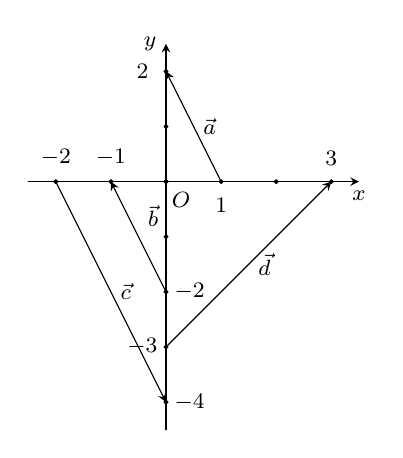
\begin{tikzpicture}[scale=.7, font=\footnotesize, line join=round, line cap=round, >=stealth]
			\draw[->] (-2.5,0)--(3.5,0) node[below] {$x$};
			\draw[->] (0,-4.5)--(0,2.5) node[left] {$y$};
			\draw (0,0) node[shift={{(-50:.3)}}] {$O$};
			\foreach \x in {-2,-1,...,3}
			\draw[fill=black] (\x,0) circle(1pt);
			\foreach \y in {-4,-3,...,2}
			\draw[fill=black] (0,\y) circle(1pt);
			\draw[->] (1,0)--(0,2) node[right, pos=0.5] {$\vec{a}$};
			\draw[->] (0,-2)--(-1,0) node[above right, pos=0.5] {$\vec{b}$};
			\draw[->] (-2,0)--(0,-4) node[right, pos=0.5] {$\vec{c}$};
			\draw[->] (0,-3)--(3,0) node[right, pos=0.5] {$\vec{d}$};
			\foreach \a/\b in {-2/90,-1/90,1/-90,3/90}
			\draw (\a,0) node[shift={{(\b:.3)}}] {$\a$};%vẽ số trục hoành
			\foreach \a/\b in {-4/0,-3/180,-2/0,2/180}
			\draw (0,\a) node[shift={{(\b:.3)}}] {$\a$};% vẽ số trục tung
		\end{tikzpicture}
	}
	\loigiai{
		Dựa vào hình vẽ ta thấy
		\begin{itemize}
			\item Các vectơ cùng phương là $\vec{a}$, $\vec{b}$ và $\vec{c}$.
			\item Các cặp vectơ ngược hướng là $\vec{a}$ với $\vec{c}$ và $\vec{b}$ với $\vec{c}$.
			\item Các cặp vectơ bằng nhau là $\vec{a}$ với $\vec{b}$.
		\end{itemize}
		
	}
\end{vd}

% \begin{vd}%[Đăng Tạ, Dự án bài giảng 10, 2022]
% 	Cho hình vuông $ABCD$. Hãy chỉ ra mối quan hệ về độ dài, phương, hướng giữa các cặp vectơ
% 	\begin{enumEX}{3}
% 		\item $\overrightarrow{AB}$ và $\overrightarrow{DC}$.
% 		\item $\overrightarrow{AD}$ và $\overrightarrow{CB}$.
% 		\item $\overrightarrow{AC}$ và $\overrightarrow{BD}$.
% 	\end{enumEX}
% 	Những cặp vectơ nào trong các cặp vectơ trên là bằng nhau?
% 	\loigiai{
% 		\immini{
% 			\begin{enumerate}
% 				\item Hai vectơ $\overrightarrow{AB}$ và $\overrightarrow{DC}$ cùng độ dài và cùng hướng. Do đó, hai $\overrightarrow{AB}$ và $\overrightarrow{DC}$ bằng nhau.
% 				\item Hai vectơ $\overrightarrow{AD}$ và $\overrightarrow{CB}$ cùng độ dài và ngược hướng. Do đó, hai $\overrightarrow{AD}$ và $\overrightarrow{CB}$ không bằng nhau.
% 				\item Hai vectơ $\overrightarrow{AC}$ và $\overrightarrow{BD}$ cùng độ dài nhưng không cùng phương nên không cùng hướng. Do đó, hai $\overrightarrow{AC}$ và $\overrightarrow{BD}$ không bằng nhau.
% 			\end{enumerate}	
% 		}{
% 			\begin{tikzpicture}[scale=1, font=\footnotesize, line join=round, line cap=round, >=stealth]
% 				\coordinate (A) at (0,0);
% 				\coordinate (B) at (0,4);
% 				\coordinate (D) at (4,0);
% 				\coordinate (C) at ($(B)+(D)-(A)$);
% 				\foreach \a/\b in {A/-90,B/90,C/90,D/-90}
% 				\draw[fill=black] (\a) circle (1pt) node[shift={{(\b:.3)}}] {$\a$};
% 				\foreach \x/\y in {A/B, D/C, A/D, C/B, A/C, B/D}
% 				\draw[->,line width=1 pt] (\x)--(\y);
% 			\end{tikzpicture}
% 		}
% 	}
% \end{vd}

\begin{vd}%[Đăng Tạ, Dự án bài giảng 10, 2022]
	Cho hình bình hành $ABCD$ có tâm là $O$ . Hãy tìm các cặp vectơ khác $\overrightarrow{0}$, bằng nhau và 
	\begin{enumerate}
		\item có điểm đầu và điểm cuối trong các điểm $A$ , $B$ , $C$ và $D$ .
		\item có điểm đầu là $O$ hoặc điểm cuối là $O$.
	\end{enumerate}
	\loigiai{
		\immini{
			\begin{enumerate}
				\item Các cặp vectơ khác $\overrightarrow{0}$, bằng nhau và có điểm đầu và điểm cuối trong các điểm $A$ , $B$ , $C$ và $D$: $\overrightarrow{AB}$ và $\overrightarrow{DC}$, $\overrightarrow{BA}$ và $\overrightarrow{CD}$, $\overrightarrow{BC}$ và $\overrightarrow{AD}$, $\overrightarrow{CB}$ và $\overrightarrow{DA}$.
				\item Các cặp vectơ khác $\overrightarrow{0}$, bằng nhau và có điểm đầu là $O$ hoặc điểm cuối là $O$: $\overrightarrow{OA}$ và $\overrightarrow{CO}$, $\overrightarrow{AO}$ và $\overrightarrow{OC}$, $\overrightarrow{OB}$ và $\overrightarrow{DO}$, $\overrightarrow{BO}$ và $\overrightarrow{OD}$.
			\end{enumerate}	
		}{
			\begin{tikzpicture}[scale=1, font=\footnotesize, line join=round, line cap=round, >=stealth]
				\coordinate (A) at (0,0);
				\coordinate (B) at (1,3);
				\coordinate (D) at (4,0);
				\coordinate (C) at ($(B)+(D)-(A)$);
				\coordinate (O) at ($(B)!0.5!(D)$);
				\foreach \a/\b in {A/-90,B/90,C/90,D/-90,O/0}
				\draw[fill=black] (\a) circle (1pt) node[shift={{(\b:.3)}}] {$\a$};
				\draw (C)--(A)--(B)--(C)--(D)--(B) (A)--(D);
			\end{tikzpicture}
		}
	}
\end{vd}

% \begin{vd}%[Đăng Tạ, Dự án bài giảng 10, 2022]
% 	Hai ca nô A và B chạy trên cùng khúc sông (khúc sông thẳng) với cùng độ lớn vận tốc là $15$ km/h. Tuy vậy, ca nô A chạy xuôi dòng, ca nô B chạy ngược dòng. Vận tốc dòng nước là $5$ km/h.
% 	\begin{enumerate}
% 		\item Hãy thể hiện bằng hình vẽ, vectơ vận tốc $\vec{v}$ dòng nước và vectơ vận tốc thực tế $\overrightarrow{v_A}$, $\overrightarrow{v_B}$ của hai ca nô A và B.
% 		\item Trong các vectơ $\vec{v}$, $\overrightarrow{v_A}$, $\overrightarrow{v_B}$ những vectơ nào cùng phương, những cặp vectơ nào ngược hướng.
% 	\end{enumerate}
% 	\loigiai{
% 		\begin{enumerate}
% 			\item 
			
% 			\immini{	
% 				\begin{itemize}
% 					\item Vì $A$ chạy xuôi dòng nên $$\left|\overrightarrow{v_A}\right|=15+5 = 20.$$
% 					\item Vì $B$ chạy ngược dòng nên $$\left|\overrightarrow{v_B}\right|=15-5 = 10.$$
% 				\end{itemize}
% 			}{
% 				\begin{tikzpicture}[scale=1, font=\footnotesize, line join=round, line cap=round, >=stealth]
% 					\draw[line width = 0.2 pt, dashed] (0,0) grid (8,5);
% 					\draw (0,2) circle(6pt) node {A};
% 					\draw[->, line width = 2pt, blue] (0,2)--(4,2) node[pos=0.4, above] {$\overrightarrow{v_A}$};
% 					\draw (8,2) circle(6pt) node {B};
% 					\draw[->, line width = 2pt, red] (8,2)--(6,2) node[pos=0.3, above] {$\overrightarrow{v_B}$};
% 					\draw[->, line width = 2pt, black] (2,4)--(3,4) node[pos=0.5, above] {$\vec{v}$};
% 					%chú thích độ dài
% 					\draw[line width=2] (6,4)--(7,4) node[pos=0.5,above] {$5$km/h};
% 					\draw[line width=2] (6,4+0.1)--(6,4-0.1);
% 					\draw[line width=2] (7,4+0.1)--(7,4-0.1);
% 				\end{tikzpicture}
% 			}
			
% 			\item Dựa vào hình vẽ ta thấy
% 			\begin{itemize}
% 				\item Các vectơ cùng phương là $\vec{v}$, $\overrightarrow{v_A}$, $\overrightarrow{v_B}$.
% 				\item Các cặp vectơ ngược hướng là $\vec{v}$ và $\overrightarrow{v_B}$, $\overrightarrow{v_A}$ và $\overrightarrow{v_B}$.
% 			\end{itemize}
% 		\end{enumerate}
% 	}
% \end{vd}

\baitaptl
\setcounter{bt}{0}

\begin{bt}%[Đăng Tạ, Dự án bài giảng 10, 2022]
	\immini{Cho hình vẽ, hãy chỉ ra các vectơ cùng phương, các cặp vectơ ngược hướng và các cặp vectơ bằng nhau }{
		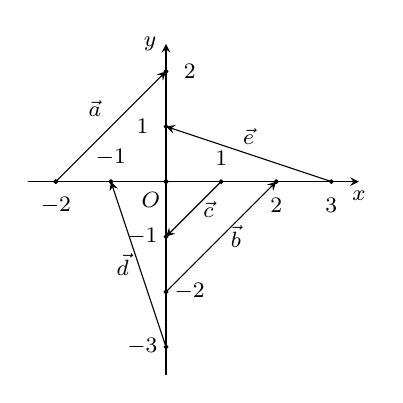
\begin{tikzpicture}[scale=.7, font= \footnotesize, line join=round, line cap=round, >=stealth]
			\draw[->] (-2.5,0)--(3.5,0) node[below] {$x$};
			\draw[->] (0,-3.5)--(0,2.5) node[left] {$y$};
			\draw (0,0) node[shift={{(-130:.3)}}] {$O$};
			\foreach \x in {-2,-1,...,3}
			\draw[fill=black] (\x,0) circle(1pt);
			\foreach \y in {-3,-2,...,2}
			\draw[fill=black] (0,\y) circle(1pt);
			\draw[->] (-2,0)--(0,2) node[above left, pos=0.5] {$\vec{a}$};
			\draw[->] (0,-2)--(2,0) node[right, pos=0.5] {$\vec{b}$};
			\draw[->] (1,0)--(0,-1) node[right, pos=0.5] {$\vec{c}$};
			\draw[->] (0,-3)--(-1,0) node[left, pos=0.5] {$\vec{d}$};
			\draw[->] (3,0)--(0,1) node[above, pos=0.5] {$\vec{e}$};
			\foreach \a/\b in {-2/-90,-1/90,1/90, 2/-90, 3/-90}
			\draw (\a,0) node[shift={(\b:.3)}] {$\a$};%vẽ số trục hoành
			\foreach \a/\b in {-3/180,-2/0, -1/180, 1/180, 2/0}
			\draw (0,\a) node[shift={(\b:.3)}] {$\a$};% vẽ số trục tung
		\end{tikzpicture}
	}
	\loigiai{
		Dựa vào hình vẽ ta thấy
		\begin{itemize}
			\item Các vectơ cùng phương là $\vec{a}$, $\vec{b}$ và $\vec{c}$.
			\item Các cặp vectơ ngược hướng là $\vec{a}$ với $\vec{c}$ và $\vec{b}$ với $\vec{c}$.
			\item Các cặp vectơ bằng nhau là $\vec{a}$ với $\vec{b}$.
		\end{itemize}
		
	}
\end{bt}

\begin{bt}%[Đăng Tạ, Dự án bài giảng 10, 2022]
	Cho tam giác đều $ABC$, hãy chỉ ra mối quan hệ về độ dài, phương và hướng giữa cặp vectơ $\overrightarrow{BA}$ và $\overrightarrow{CA}$. Hai vectơ có bằng nhau không?
	\loigiai{
		\immini{
			Dựa vào hình vẽ ta thấy hai vectơ $\overrightarrow{BA}$ và $\overrightarrow{CA}$ cùng độ dài nhưng không cùng phương nên cũng không cùng hướng. Do đó, hai vectơ $\overrightarrow{BA}$ và $\overrightarrow{CA}$ không bằng nhau.
		}{
			\begin{tikzpicture}[scale=1, font=\footnotesize, line join=round, line cap=round, >=stealth]
				\coordinate (B) at (0,0);
				\coordinate (C) at (3.5,0);
				\tkzDefEquilateral(B,C)    \tkzGetPoint{A}
				\draw[->,line width=1 pt] (B)--(A);
				\draw[->,line width=1 pt] (C)--(A);
				\draw (B)--(C);
				\foreach \p/\g in {A/90, B/-90, C/-90}
				\draw[fill=black] (\p) circle(1pt) node [shift={(\g:.3)}] {$\p$};
			\end{tikzpicture}	
			
		}
		
	}
\end{bt}

\begin{bt}%[Đăng Tạ, Dự án bài giảng 10, 2022]
	\immini{Cho hình lục giác đều $ABCDEF$ có tâm $O$.
		\begin{enumerate}
			\item Hãy tìm các vectơ khác $\overrightarrow{0}$ và bằng với $\overrightarrow{AB}$.
			\item Hãy vẽ vectơ bằng với $\overrightarrow{AE}$ và có điểm đầu là $B$.
			\item Hãy vẽ vectơ bằng với $\overrightarrow{AE}$ và có điểm đầu là $C$.
	\end{enumerate}}
	{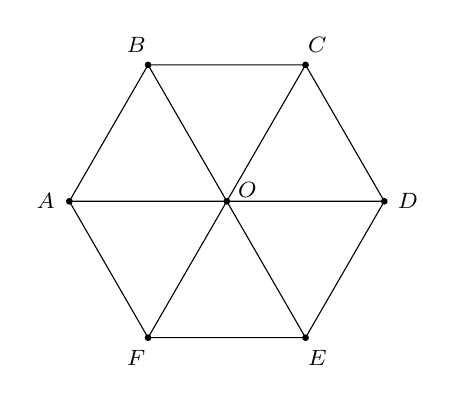
\begin{tikzpicture}[scale=1, font=\footnotesize, line join=round, line cap=round, >=stealth]
			\coordinate (O) at (0,0);
			\foreach \x/\y in {A/180,B/120,C/60,D/0,E/-60,F/-120} {
				\coordinate (\x) at (\y:2);
				\draw[fill=black] (\x) circle(1pt) node [shift={(\y:.3)}] {$\x$};}
			\draw[fill=black] (O) circle(1pt) node[shift={(30:.3)}] {$O$};
			\draw (A)--(B)--(C)--(D)--(E)--(F)--cycle;
			\draw (A)--(D) (B)--(E) (C)--(F);
	\end{tikzpicture}}
	\loigiai{
		\immini{
			\begin{enumerate}
				\item các vectơ khác $\vec{0}$ và bằng với vectơ $\overrightarrow{AB}$ là $\overrightarrow{FO}$, $\overrightarrow{OC}$, $\overrightarrow{ED}$.
				\item Vì $ABDE$ là tứ giác có hai đường chéo cắt nhau tại mỗi đường nên là hình bình hành. Suy ra, vectơ bằng với $\overrightarrow{AE}$ có điểm đầu $B$ là $\overrightarrow{BD}$.
				\item Giả sử $\overrightarrow{CG}$ là vectơ cần dựng và vì $\overrightarrow{CG}=\overrightarrow{AE}$ nên $AEGC$ là hình bình hành.
			\end{enumerate}
			
		}{
			\begin{tikzpicture}[scale=1, font=\footnotesize, line join=round, line cap=round, >=stealth]
				\coordinate (O) at (0,0);
				\foreach \x/\y in {A/180,B/120,C/60,D/0,E/-60,F/-120} {
					\coordinate (\x) at (\y:2);
					\draw[fill=black] (\x) circle(1pt) node [shift={(\y:.3)}] {$\x$};}
				\draw[fill=black] (O) circle(1pt) node[shift={(30:.3)}] {$O$};
				\draw (A)--(B)--(C)--(D)--(E)--(F)--cycle;
				\draw (A)--(D) (B)--(E) (C)--(F);
				\coordinate (G) at ($(C)+(E)-(A)$);
				\draw[fill=black] (G) circle(1pt) node[shift={(30:.3)}] {$G$};
				\draw[->, line width = 1] (A)--(E);
				\draw[->, line width = 1] (B)--(D);
				\draw[->, line width = 1] (C)--(G);
				\draw[dashed] (A)--(C) (E)--(G);
			\end{tikzpicture}
			
		}
		\vspace*{0.2cm}
		Vậy điểm $G$ cần dựng là đỉnh còn lại của hình bình hành $AEGC$.
		
	}
\end{bt}

\begin{bt}%[Đăng Tạ, Dự án bài giảng 10, 2022]
	Chứng minh ba điểm $A$, $B$, $C$ thẳng hàng khi và chỉ khi $\overrightarrow{AB}$, $\overrightarrow{AC}$ cùng phương.
	\loigiai{
		\begin{itemize}
			\item Giả sử $A$, $B$, $C$ thẳng hàng. Khi đó, chúng cùng nằm trên một đường thẳng. Suy ra, $\overrightarrow{AB}$, $\overrightarrow{AC}$ có giá trùng nhau. Vậy $\overrightarrow{AB}$, $\overrightarrow{AC}$ cùng phương.
			\item Giả sử $\overrightarrow{AB}$, $\overrightarrow{AC}$ cùng phương. Khi đó, $\overrightarrow{AB}$, $\overrightarrow{AC}$ có giá song song hoặc trùng nhau. Mặt khác, giá của $\overrightarrow{AB}$, $\overrightarrow{AC}$ cùng đi qua điểm $A$ nên chúng trùng nhau. Vậy $A$, $B$, $C$ thẳng hàng.
		\end{itemize}
	}
\end{bt}

% \begin{bt}%[Đăng Tạ, Dự án bài giảng 10, 2022]
% 	Trên mặt phẳng $Oxy$, hãy vẽ các vectơ $\overrightarrow{OA}$ và $\overrightarrow{MN}$ với $A(1;2)$, $M(0;-1)$ và $N(3;5)$
% 	\begin{enumerate}
% 		\item Chỉ ra một mối liên hệ giữa hai vectơ trên.
% 		\item Một vật thể khởi hành từ $M$ và chuyển động thẳng đều với vận tốc (tính theo giờ) được biểu diễn bởi vectơ $\vec{v}=\overrightarrow{OA}$. Hỏi vật thể có đi qua $N$ không? Nếu có thì sau bao lâu vật sẽ đến $N$?
% 	\end{enumerate}
% 	\loigiai{
% 		\immini{
% 			\begin{enumerate}
% 				\item Dựa vào hình vẽ ta thấy hai vectơ $\overrightarrow{OA}$ và $\overrightarrow{MN}$ cùng hướng.
% 				\item Vì hai vectơ $\overrightarrow{OA}$ và $\overrightarrow{MN}$ cùng hướng nên vật thể khởi hành từ $M$ có thể đi đến $N$. \\
% 				Mặt khác, vì $\left|\overrightarrow{MN}\right|=3\left|\overrightarrow{OA}\right|=3\left|\vec{v}\right|$ nên sau $3$ giờ thì vật sẽ di chuyển đến $N$.
% 			\end{enumerate}
% 		}{
			
% 			\begin{tikzpicture}[scale=1, font=\footnotesize, line join=round, line cap=round, >=stealth]
% 				\draw[->] (-0.5,0)--(4,0) node[below] {$x$};
% 				\draw[->] (0,-1.5)--(0,6) node[right] {$y$};
% 				\draw[dashed, line width=0.3pt] (-0.5,-1.5) grid (3.5,5.5);
% 				\coordinate (A) at (1,2);
% 				\coordinate (O) at (0,0);
% 				\coordinate (M) at (0,-1);
% 				\coordinate (N) at (3,5);
% 				\draw (O) node[shift={{(-130:.3)}}] {$O$};
% 				\foreach \x in {1,2,...,3}
% 				\draw[fill=black] (\x,0) circle(1pt);
% 				\foreach \y in {-1,0,...,5}
% 				\draw[fill=black] (0,\y) circle(1pt);
% 				\draw[->, line width=2pt] (O)--(A) node[left,pos=.6]{$\vec{v}$};
% 				\draw[->, line width=2pt] (M)--(N);
% 				\foreach \a/\b in {1/-40,3/-40}
% 				\draw (\a,0) node[shift={(\b:.3)}] {$\a$};%vẽ số trục hoành
% 				\foreach \a/\b in {-1/150,2/130, 5/130}
% 				\draw (0,\a) node[shift={(\b:.3)}] {$\a$};% vẽ số trục tung
% 				\foreach \a/\b in {A/145,M/-40, N/145}
% 				\draw (\a) node[shift={(\b:.3)}] {$\a$};%vẽ tên điểm
				
% 			\end{tikzpicture}
% 		}
		
		
% 	}
% \end{bt}
\subsection{Câu hỏi trắc nghiệm}
\Opensolutionfile{ansbook}[ans/ansbook-0H4-7-TN]
\Opensolutionfile{ans}[ans/ans-0H4-7-TN]

\setcounter{ex}{0}

% \begin{ex}%[0H1Y1-1]
% 	vectơ là một đoạn thẳng
% 	\choice
% 	{\True Có hướng}
% 	{Có hướng dương và hướng âm}
% 	{Có hai đầu mút}
% 	{Thỏa mãn ba tính chất trên}
% 	\loigiai{
% 		vectơ là một đoạn thẳng có hướng.
% 	}
% \end{ex}


\begin{ex}%[0H1Y1-1]
	Chọn khẳng định đúng trong các khẳng định sau.
	\choice
	{vectơ là một đường thẳng có hướng}
	{vectơ là một đoạn thẳng}
	{\True vectơ là một đoạn thẳng có hướng}
	{vectơ là một đoạn thẳng không phân biệt điểm đầu và điểm cuối}
	\loigiai{vectơ là một đoạn thẳng có hướng.
	}
\end{ex}


% \begin{ex}%[0H1Y1-1]
% 	vectơ có điểm đầu $ D $ và điểm cuối $ E $ được kí hiệu như thế nào là đúng?
% 	\choice
% 	{$ DE $}
% 	{$ ED $}
% 	{$ \left|\overrightarrow{DE}\right| $}
% 	{\True $ \overrightarrow{DE} $}
% 	\loigiai{vectơ có điểm đầu $ D $ và điểm cuối $ E $ được kí hiệu $ \overrightarrow{DE} $.
% 	}
% \end{ex}


\begin{ex}%[0H1B1-1]
	Cho tam giác $ ABC $ có thể xác định được bao nhiêu vectơ (khác vectơ không) có điểm đầu và điểm cuối là đỉnh $ A $, $ B $, $ C $?
	\choice
	{$ 2 $}
	{$ 3 $}
	{$ 4 $}
	{\True $ 6 $}
	\loigiai{Có thể xác định được 6 vectơ (khác vectơ không) có điểm đầu và điểm cuối là đỉnh $ A $, $ B $, $ C $ là các vectơ $ \overrightarrow{AB} $, $ \overrightarrow{BA} $, $ \overrightarrow{AC} $, $ \overrightarrow{CA} $, $ \overrightarrow{BC} $, $ \overrightarrow{CB} $.
	}
\end{ex}


\begin{ex}%[0H1B1-1]
	Cho hai điểm phân biệt $ A $, $ B $. Số vectơ (khác $ \overrightarrow{0} $) có điểm đầu và điểm cuối lấy từ các điểm $ A $, $ B $ là
	\choice
	{\True $ 2 $}
	{$ 6 $}
	{$ 13 $}
	{$ 12 $}
	\loigiai{Có 2 vectơ có điểm đầu và điểm cuối lấy từ các điểm $ A $, $ B $ là $ \overrightarrow{AB} $ và $ \overrightarrow{BA} $.
	}
\end{ex}


% \begin{ex}%[0H1K1-1]
% 	Số vectơ (khác $ \overrightarrow{0} $) có điểm đầu và điểm cuối lấy từ 7 điểm phân biệt cho trước (3 điểm bất kì không thẳng hàng) là 
% 	\choice
% 	{\True $ 42 $}
% 	{$ 3 $}
% 	{$ 9 $}
% 	{$ 27 $}
% 	\loigiai{
% 		Cứ $1$ điểm tạo với $6$ điểm còn lại ta được $6$ vectơ.\\
% 		Vậy có tất cả $6\cdot 7=42$ vectơ tạo thành.
% 	}
% \end{ex}


% \begin{ex}%[0H1B1-1]
% 	Cho tứ giác $ ABCD $. Có thể xác định được bao nhiêu vectơ (khác $ \overrightarrow{0} $) có điểm đầu và điểm cuối là các điểm $ A $, $ B $, $ C $, $ D $?
% 	\choice
% 	{$ 4 $}
% 	{$ 8 $}
% 	{$ 10 $}
% 	{\True $ 12 $}
% 	\loigiai{Có thể xác định được 12 vectơ (khác $ \overrightarrow{0} $) có điểm đầu và điểm cuối là các điểm $ A $, $ B $, $ C $, $ D $ là các vectơ $ \overrightarrow{AB} $, $ \overrightarrow{AC} $, $ \overrightarrow{AD} $, $ \overrightarrow{BC} $, $ \overrightarrow{BD} $, $ \overrightarrow{CD} $ và các vectơ đối của chúng.
% 	}
% \end{ex}



% \begin{ex}%[0H1B1-1]
% 	Cho vectơ có điểm đầu và điểm cuối trùng nhau. Khẳng định nào dưới đây \textbf{sai}?
% 	\choice
% 	{Được gọi là vectơ suy biến}
% 	{Được gọi là vectơ có phương tùy ý}
% 	{Được gọi là vectơ không, kí hiệu là $ \overrightarrow{0} $}
% 	{\True Là vectơ có độ dài không xác định}
% 	\loigiai{vectơ có điểm đầu và điểm cuối trùng nhau có độ dài là $ 0 $.	
% 	}
% \end{ex}



\begin{ex}%[0H1B1-3] 
	Cho tam giác đều $ ABC $. Mệnh đề nào sau đây \textbf{sai}?
	\choice
	{\True $ \overrightarrow{AB}=\overrightarrow{BC} $}
	{$ \overrightarrow{AC} \ne \overrightarrow{BC} $}
	{$ \left|\overrightarrow{AB}\right| =\left|\overrightarrow{BC}\right|$}
	{$ \overrightarrow{AC} $ không cùng phương $ \overrightarrow{BC} $}
	\loigiai{\immini{Có $ \overrightarrow{AB}$ và $\overrightarrow{BC} $ là 2 vectơ không cùng phương nên $ \overrightarrow{AC} \ne \overrightarrow{BC} $.}{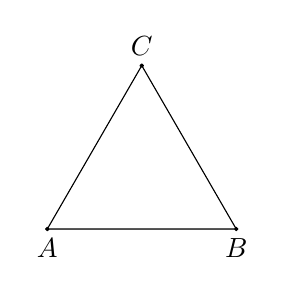
\begin{tikzpicture}[>=stealth, line join = round, line  cap = round,scale=0.6]
				\draw[fill] (0,0) node[below]{$ A $} circle(1pt)-- (4,0) node[below]{$ B $} circle(1pt) -- (2,3.46) node[above]{$ C $} circle(1pt) --(0,0);
		\end{tikzpicture}}
	}
\end{ex}


\begin{ex}%[0H1Y1-3]
	Khẳng định nào dưới đây là \textbf{sai}?
	\choice
	{Mỗi vectơ đều có một độ dài, đó là khoảng cách giữa điểm đầu và điểm cuối của vectơ đó}
	{Độ dài của vectơ $ \overrightarrow{a} $ được kí hiệu là $ \left|\overrightarrow{a}\right| $}
	{\True $ \left|\overrightarrow{PQ}\right|=\overrightarrow{PQ} $}
	{$ \left|\overrightarrow{AB}\right| =AB=BA$}
	\loigiai{$ \left|\overrightarrow{PQ}\right|$ khác $\overrightarrow{PQ} $ do vectơ là một đoạn thẳng định hướng còn độ dài vectơ là độ dài đoạn thẳng nối điểm đầu và điểm cuối vectơ đó.
	}
\end{ex}


% \begin{ex}%[0H1B1-3] 
% 	Cho tam giác đều $ ABC $, cạnh $ a $. Mệnh đề nào sau đây đúng?
% 	\choice
% 	{$ \overrightarrow{AC}=a $}
% 	{$ \left|\overrightarrow{AC}\right|=\overrightarrow{BC} $}
% 	{\True $ \left|\overrightarrow{AB}\right|=a $}
% 	{$ \overrightarrow{AB} $ cùng hướng với $ \overrightarrow{BC} $}
% 	\loigiai{\immini{Có $ \left|\overrightarrow{AB} \right|=AB=a$.}{\begin{tikzpicture}[>=stealth, line join = round, line  cap = round,scale=0.6]
% 				\draw[fill] (0,0) node[below]{$ A $} circle(1pt)-- (4,0) node[below]{$ B $} circle(1pt) -- (2,3.46) node[above]{$ C $} circle(1pt) --(0,0);
% 		\end{tikzpicture}}
% 	}
% \end{ex}

% \begin{ex}%[0H1B1-3]
% 	Cho tam giác $ABC$ đều cạnh $a$. Gọi $M$ là trung điểm $BC$. Khẳng định nào sau đây đúng?
% 	\choice
% 	{\True $\left| \overrightarrow{AM}\right|=\dfrac{a\sqrt{3}}{2}$}
% 	{$\overrightarrow{AM}=a$}
% 	{$\overrightarrow{AM}=\dfrac{a\sqrt{3}}{2}$}
% 	{$\overrightarrow{MB}=\overrightarrow{MC}$}
% 	\loigiai{
% 		Ta có $AM$ là đường trung tuyến tam giác đều  suy ra $\left|\overrightarrow{AM}\right|=AM=\dfrac{a\sqrt{3}}{2}$.
% 	}
% \end{ex}

\begin{ex}%[0H1B1-3]
	Cho tam giác $ABC$. Gọi $M,N$ lần lượt là trung điểm các cạnh $AB$, $AC$. Mệnh đề nào sau đây \textbf{sai}?
	\choice
	{\True $\overrightarrow{BC}=2\overrightarrow{NM}$}
	{$\overrightarrow{MN}=\dfrac{1}{2}\overrightarrow{BC}$}
	{$\overrightarrow{AN}=\overrightarrow{NC}$}
	{$\left|\overrightarrow{MA}\right|=\left|\overrightarrow{MB}\right|$}
	\loigiai{
		\immini{
			$\bullet$ $\overrightarrow{AN}=\overrightarrow{NC}$ đúng vì $\overrightarrow{AN}$ và $\overrightarrow{NC}$ cùng hướng và cùng độ dài.\\
			$\bullet$ $\overrightarrow{MN}=\dfrac{1}{2}\overrightarrow{BC}$ đúng vì $MN$ là đường trung bình của $\Delta ABC$ nên $MN=\dfrac{1}{2}BC$ và $\overrightarrow{MN}$, $\overrightarrow{BC}$ cùng hướng.\\
			$\bullet$ $\left|\overrightarrow{MA}\right|=\left|\overrightarrow{MB}\right|$ đúng vì $M$ là trung điểm $AB$ nên $MA=MB$.\\
			$\bullet$ $\overrightarrow{BC}=2\overrightarrow{NM}$ sai vì mệnh đề đúng tương ứng là $\overrightarrow{BC}=2\overrightarrow{MN}$.
		}{\begin{tikzpicture}[>=stealth, line join = round, line  cap = round,scale=0.6]
				\tkzInit[ymin=-1,ymax=10,xmin=-1,xmax=15]
				\tkzSetUpPoint[color=black,fill=black,size=2]
				\tkzDefPoints{3/5/A,1/0/B,7/0/C}
				\tkzDefMidPoint(A,B)
				\tkzGetPoint{M}
				\tkzDefMidPoint(A,C)
				\tkzGetPoint{N}
				\tkzDrawSegments(A,B B,C C,A A,N N,C M,N M,A M,B)
				\tkzDrawPoints(A,B,C,M,N)
				\tkzLabelPoints[left](A,B,M)
				\tkzLabelPoints[right](C,N)
		\end{tikzpicture}}
	}
\end{ex}


\begin{ex}%[0H1B1-2]
	Cho hai vectơ không cùng phương $\overrightarrow{a}$ và $\overrightarrow{b}$. Khẳng định nào sau đây đúng?
	\choice
	{Không có vectơ nào cùng phương với cả hai vectơ $\overrightarrow{a}$ và $\overrightarrow{b}$}
	{Có vô số vectơ cùng phương với cả hai vectơ $\overrightarrow{a}$ và $\overrightarrow{b}$}
	{\True Có một vectơ cùng phương với cả hai vectơ $\overrightarrow{a}$ và $\overrightarrow{b}$}
	{Có hai vectơ cùng phương với cả hai vectơ $\overrightarrow{a}$ và $\overrightarrow{b}$}
	\loigiai{
		Có một vectơ cùng phương với cả hai vectơ $\overrightarrow{a}$ và $\overrightarrow{b}$ đó là vectơ không.
	}
\end{ex}

\begin{ex}%[0H1B1-2]
	Cho $3$ điểm phân biệt $A$, $B$, $C$. Khi đó khẳng định nào sau đây {\bf sai}?
	\choice
	{$A$, $B$, $C$ thẳng hàng khi và chỉ khi $\overrightarrow{AB}$ và $\overrightarrow{AC}$ cùng phương}
	{$A$, $B$, $C$ thẳng hàng khi và chỉ khi $\overrightarrow{AB}$ và $\overrightarrow{BC}$ cùng phương}
	{$A$, $B$, $C$ thẳng hàng khi và chỉ khi $\overrightarrow{AC}$ và $\overrightarrow{BC}$ cùng phương}
	{\True $A$, $B$, $C$ thẳng hàng khi và chỉ khi $AC=BC$}
	\loigiai{
		$A$, $B$, $C$ thẳng hàng khi và chỉ khi các vectơ $\overrightarrow{AB}$, $\overrightarrow{AC}$, $\overrightarrow{BC}$ đôi một cùng phương.
	}
\end{ex}

\begin{ex}%[0H1B1-2]
	Mệnh đề nào sau đây đúng?
	\choice
	{\True Có duy nhất một vectơ cùng phương với mọi vectơ}
	{Có ít nhất hai vectơ cùng phương với mọi vectơ}
	{Có vô số vectơ cùng phương với mọi vectơ}
	{Không có vectơ nào cùng phương với mọi vectơ}
	\loigiai{
		Có duy nhất một vectơ cùng phương với mọi vectơ đó là vectơ không.	
	}
\end{ex}


\begin{ex}%[0H1B1-2]
	Khẳng định nào sau đây đúng?
	\choice
	{Hai vectơ cùng phương với một vectơ thứ ba thì cùng phương}
	{\True Hai vectơ cùng phương với một vectơ thứ ba khác $\overrightarrow{0}$ thì cùng phương}
	{vectơ không là vectơ không có giá}
	{Điều kiện đủ để hai vectơ bằng nhau là chúng có độ dài bằng nhau}
	\loigiai{
		Hai vectơ cùng phương với một vectơ thứ ba khác $\overrightarrow{0}$ thì cùng phương.
	}
\end{ex}

\begin{ex}%[0H1Y1-2]
	Cho lục giác đều $ABCDEF$ tâm $O$. Số các vectơ khác $\overrightarrow{0}$ cùng phương với $\overrightarrow{OC}$ có điểm đầu và điểm cuối là các đỉnh của lục giác bằng
	\choice
	{\True $6$}
	{$7$}
	{$8$}
	{$4$}
	\loigiai{
		\immini{
			Số các vectơ khác $\overrightarrow{0}$ cùng phương với $\overrightarrow{OC}$ có điểm đầu và điểm cuối là các đỉnh của lục giác là 
			$\overrightarrow{AB}$, $\overrightarrow{BA}$, $\overrightarrow{FC}$, $\overrightarrow{CF}$, $\overrightarrow{ED}$, $\overrightarrow{DE}$.
		}
		{
			\begin{tikzpicture}[>=stealth, line join = round, line  cap = round,scale=0.8]
				\tkzDefPoints{0/0/O, 3/0/A}
				\tkzDefPointBy[rotation = center O angle 60](A)    \tkzGetPoint{B}
				\tkzDefPointBy[rotation = center O angle 120](A)    \tkzGetPoint{C}
				\tkzDefPointBy[rotation = center O angle 180](A)    \tkzGetPoint{D}
				\tkzDefPointBy[rotation = center O angle 60](D)    \tkzGetPoint{E}
				\tkzDefPointBy[rotation = center O angle 1200](D)    \tkzGetPoint{F}
				\tkzDrawSegments(O,A O,B O,C O,D O,E O,F A,B B,C C,D D,E E,F F,A)
				\tkzDrawPoints[size=2](O,A,B,C,D,E,F)
				\node[] at (0.5,0.23) {O};
				\tkzLabelPoints[above](C,B)
				\tkzLabelPoints[below](E,F)
				\tkzLabelPoints[right](A)
				\tkzLabelPoints[left](D)
			\end{tikzpicture}
		}
	}
\end{ex}

\begin{ex}%[0H1B1-2]
	Cho ba điểm $ A $, $ B $, $ C $ phân biệt. Khi đó
	\choice
	{\True Điều kiện cần và đủ để $ A $, $ B $, $ C $ thẳng hàng là $ \overrightarrow{AC} $ cùng phương với $ \overrightarrow{AB} $}
	{Điều kiện đủ để $ A $, $ B $, $ C $ thẳng hàng là $ \overrightarrow{CA} $ cùng phương với $ \overrightarrow{AB} $}
	{Điều kiện cần để $ A $, $ B $, $ C $ thẳng hàng là $ \overrightarrow{CA} $ cùng phương với $ \overrightarrow{AB} $}
	{Điều kiện cần và đủ để $ A $, $ B $, $ C $ thẳng hàng là $ \overrightarrow{AB} = \overrightarrow{AC} $}
	\loigiai{Điều kiện cần và đủ để $ A $, $ B $, $ C $ thẳng hàng là $ \overrightarrow{AC} $ cùng phương với $ \overrightarrow{AB} $.
	}
\end{ex}

% \begin{ex}%[0H1B1-2]
% 	Trong mặt phẳng tọa độ $O x y$, cho $\overrightarrow{a} = (-3; 0)$, $\overrightarrow{b} = (4; x)$. Giá trị của $x$ để $\overrightarrow{a}$ và $\overrightarrow{b}$ cùng phương là
% 	\choice
% 	{$x = - \dfrac{3}{4}$}
% 	{$x = - \dfrac{4}{3}$}
% 	{\True $x=0$}
% 	{$x \in \varnothing$}
% 	\loigiai{
% 		$\overrightarrow{a}$ và $\overrightarrow{b}$ cùng phương khi tồn tại số thực $k$ khác $0$ sao cho $\overrightarrow{b} = k \overrightarrow{a} \Leftrightarrow \heva{& 4 = k . (-3) \\ & x = k . 0 } \Leftrightarrow x=0$.
% 	}
% \end{ex}


% \begin{ex}%[0H1Y1-2]
% 	Phát biểu nào sau đây là \textbf{sai}?
% 	\choice
% 	{\True Hai vectơ cùng phương thì cùng hướng}
% 	{vectơ không cùng phương với mọi vectơ}
% 	{Hai vectơ cùng hướng thì cùng phương}
% 	{vectơ là đoạn thẳng có hướng}
% 	\loigiai{
% 		Hai vectơ cùng phương có thể khác hướng. Do đó mệnh đề \lq\lq Hai vectơ cùng phương thì cùng hướng \rq\rq\, là sai.}
% \end{ex}

\begin{ex}%[0H1B1-2]
	Cho vectơ $\overrightarrow{MN}\neq \overrightarrow{0}$. Số vectơ cùng hướng với vectơ $\overrightarrow{MN}$ là
	\choice
	{\True vô số}
	{$1$}
	{$3$}
	{$2$}
	\loigiai
	{Có vô số vectơ cùng hướng với một vectơ khác vectơ-không cho trước.}
\end{ex}

\begin{ex}%[0H1B1-3] 
	Gọi $ C $ là trung điểm của đoạn $ AB $. Hãy chọn khẳng định đúng trong các khẳng định sau.
	\choice
	{$ \overrightarrow{CA}=\overrightarrow{CB} $}
	{\True $ \overrightarrow{AB} $ và $ \overrightarrow{AC} $ cùng hướng}
	{$ \overrightarrow{AB} $ và $ \overrightarrow{CB} $ ngược hướng}
	{$ \left|\overrightarrow{AB}\right|=\overrightarrow{CB} $}
	\loigiai{\immini{Có $ \overrightarrow{AB} $ và $ \overrightarrow{AC} $ cùng hướng.}{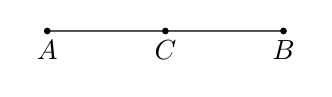
\begin{tikzpicture}[>=stealth, line join = round, line  cap = round,scale=1]
				\draw[fill] (0,0) node[below]{$ A $} circle(1pt)-- (1.5,0) node[below]{$ C $} circle(1pt) -- (3,0) node[below]{$ B $} circle(1pt);
		\end{tikzpicture}}
	}
\end{ex}


\begin{ex}%[0H1B1-2] 
	Cho ba điểm $ M $, $ N $, $ P $ thẳng hàng, trong đó điểm $ N $ nằm giữa hai điểm $ M $ và $ P $. Khi đó các cặp vectơ nào cùng hướng?
	\choice
	{$ \overrightarrow{MP} $ và $ \overrightarrow{PN} $}
	{$ \overrightarrow{MN} $ và $ \overrightarrow{PN} $}
	{$ \overrightarrow{NM} $ và $ \overrightarrow{NP} $}
	{\True $ \overrightarrow{MN} $ và $ \overrightarrow{MP} $}
	\loigiai{
		\immini{Cặp vectơ $ \overrightarrow{MN} $ và $ \overrightarrow{MP} $ là cùng hướng.}{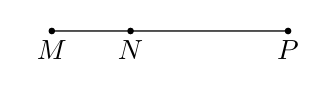
\begin{tikzpicture}[>=stealth, line join = round, line  cap = round,scale=1]
				\draw[fill] (0,0) node[below]{$ M $} circle(1pt)-- (1,0) node[below]{$ N $} circle(1pt) -- (3,0) node[below]{$ P $} circle(1pt);
		\end{tikzpicture}}
	}
\end{ex}

% \begin{ex}%[0H1Y1-2]
% 	Cho hình bình hành $ABCD$. Chọn khẳng định đúng?
% 	\choice
% 	{$\overrightarrow{AD}$, $\overrightarrow{BC}$ là hai vectơ ngược hướng}
% 	{$\overrightarrow{AD}$, $\overrightarrow{CB}$ là hai vectơ cùng hướng}
% 	{\True $\overrightarrow{AB}$, $\overrightarrow{CD}$ là hai vectơ cùng phương}
% 	{$\overrightarrow{AB}$, $\overrightarrow{CD}$ là hai vectơ cùng hướng}
% 	\loigiai{
% 		Vì $ABCD$ là hình bình hành nên $\overrightarrow{AB}$, $\overrightarrow{CD}$ là hai vectơ cùng phương.
% 	}
% \end{ex}

% \begin{ex}%[0H1B1-2]
% 	Cho hình bình hành $ABCD$. Hai vectơ nào ngược hướng?
% 	\choice
% 	{$\overrightarrow{AB}$ và $\overrightarrow{DB}$}
% 	{$\overrightarrow{AB}$ và $\overrightarrow{AC}$}
% 	{\True $\overrightarrow{AB}$ và $\overrightarrow{CD}$}
% 	{$\overrightarrow{AB}$ và $\overrightarrow{DC}$}
% 	\loigiai{
% 		\begin{center}
% 			\begin{tikzpicture}[>=stealth, line join = round, line  cap = round,scale=1]
% 				\tkzDefPoints{2/2/A,0/0/B,4/0/C}
% 				\tkzDefPointBy[translation=from B to C](A) \tkzGetPoint{D}
% 				\tkzDrawSegments(A,B B,C C,D D,A)
% 				\tkzDrawPoints[fill,size=2](A,B,C,D)
% 				\tkzLabelPoints[below](B,C)
% 				\tkzLabelPoints[above](A,D)
% 			\end{tikzpicture}
% 		\end{center}
% 		Hai vectơ $\overrightarrow{AB}$ và $\overrightarrow{CD}$ ngược hướng.
% 	}
% \end{ex}

% \begin{ex}%[0H1Y1-2]
% 	vectơ $-2\overrightarrow{a}$ và vectơ $\overrightarrow{a}$ với $\overrightarrow{a} \ne 0$ là hai vectơ
% 	\choice
% 	{\True ngược hướng}
% 	{bằng nhau}
% 	{cùng hướng}
% 	{đối nhau}
% 	\loigiai{
% 		vectơ $-2\overrightarrow{a}$ và vectơ $\overrightarrow{a}$ với $\overrightarrow{a} \ne 0$ là hai vectơ ngược hướng.
% 	}
% \end{ex}

% \begin{ex}%[0H1B1-2]
% 	Khẳng định nào sau đây đúng?
% 	\choice
% 	{\True $\overrightarrow{a} =\left(1;2\right)$ và $\overrightarrow{b}=\left(3;6\right)$ cùng hướng}
% 	{$\overrightarrow{a} =\left(1;2\right)$ và $\overrightarrow{b}=\left(2;1\right)$ đối nhau}
% 	{$\overrightarrow{a} =\left(1;2\right)$ và $\overrightarrow{b}=\left(-3;-6\right)$ cùng hướng}
% 	{$\overrightarrow{a} =\left(1;2\right)$ và $\overrightarrow{b}=\left(-3;0\right)$ cùng phương}
% 	\loigiai
% 	{ Xét $\overrightarrow{a} =\left(1;2\right)$ và $\overrightarrow{b}=\left(3;6\right)$. Do $\overrightarrow{b}=3\overrightarrow{a} \Rightarrow \overrightarrow{a} =\left(1;2\right)$ và $\overrightarrow{b}=\left(3;6\right)$ cùng hướng.
% 	}
% \end{ex}


% \begin{ex}%[0H1Y1-3]
% 	Hai vectơ bằng nhau khi và chỉ khi
% 	\choice
% 	{\True Cùng hướng và cùng độ dài}
% 	{Cùng phương}
% 	{Cùng hướng}
% 	{Có cùng độ dài}
% 	\loigiai{
% 		Hai vectơ bằng nhau khi và chỉ khi chúng cùng hướng và cùng độ dài.
% 	}
% \end{ex}


% \begin{ex}%[0H1B1-3]
% 	Khẳng định nào sau đây đúng?
% 	\choice
% 	{\True Hai vectơ $\overrightarrow{a}$, $\overrightarrow{b}$ bằng nhau, kí hiệu $\overrightarrow{a}=\overrightarrow{b}$,  nếu chúng cùng hướng và cùng độ dài}
% 	{Hai vectơ $\overrightarrow{a}$, $\overrightarrow{b}$ bằng nhau, kí hiệu $\overrightarrow{a}=\overrightarrow{b}$,  nếu chúng cùng phương và cùng độ dài}
% 	{Hai vectơ $\overrightarrow{AB}$, $\overrightarrow{CD}$ bằng nhau khi và chỉ khi tứ giác $ABCD$ là hình bình hành}
% 	{Hai vectơ $\overrightarrow{a}$, $\overrightarrow{b}$ bằng nhau khi và chỉ khi chúng cùng độ dài}
% 	\loigiai{
% 		Hai vectơ $\overrightarrow{a}$, $\overrightarrow{b}$ bằng nhau, kí hiệu $\overrightarrow{a}=\overrightarrow{b}$,  nếu chúng cùng hướng và cùng độ dài.
% 	}
% \end{ex}

\begin{ex}%[0H1Y1-3]
	Phát biểu nào sau đây đúng?
	\choice
	{Hai vectơ không bằng nhau thì độ dài của chúng không bằng nhau}
	{Hai vectơ không bằng nhau thì độ dài của chúng không cùng phương}
	{\True Hai vectơ bằng nhau thì có giá trùng nhau hoặc song song nhau}
	{Hai vectơ có độ dài không bằng nhau thì không cùng hướng}
	\loigiai{
		Hai vectơ bằng nhau thì cùng phương nên chúng có giá trùng nhau hoặc song song nhau.	
	}
\end{ex}


% \begin{ex}%[0H1B1-3]
% 	Chọn khẳng định đúng trong các khẳng định sau
% 	\choice
% 	{Hai vectơ cùng phương thì bằng nhau}
% 	{Hai vectơ ngược hướng thì có độ dài không bằng nhau}
% 	{Hai vectơ cùng phương và cùng độ dài thì bằng nhau}
% 	{\True Hai vectơ cùng hướng và cùng độ dài thì bằng nhau}
% 	\loigiai{Hai vectơ cùng hướng và cùng độ dài thì bằng nhau.	
% 	}
% \end{ex}


\begin{ex}%[0H1B1-3]
	Cho vectơ $ \overrightarrow{a} \ne \overrightarrow{0} $. Mệnh đề nào sau đây đúng?
	\choice
	{\True Có vô số vectơ $ \overrightarrow{u} $ mà $ \overrightarrow{u}=\overrightarrow{a} $}
	{Có duy nhất một $ \overrightarrow{u} $ mà $ \overrightarrow{u}=\overrightarrow{a} $}
	{Có duy nhất một $ \overrightarrow{u} $ mà $ \overrightarrow{u}=-\overrightarrow{a} $}
	{Không có vectơ $ \overrightarrow{u} $ nào mà $ \overrightarrow{u}=\overrightarrow{a} $}
	\loigiai{Có vô số vectơ $ \overrightarrow{u} $ mà $ \overrightarrow{u}=\overrightarrow{a} $.
	}
\end{ex}

\begin{ex}%[0H1B1-3]
	Cho hình bình hành $ABCD$. Đẳng thức nào sau đây \textbf{sai}?
	\choice
	{$\left|\overrightarrow{AD}\right|=\left|\overrightarrow{BC}\right|$}
	{$\left|\overrightarrow{BC}\right|=\left|\overrightarrow{DA}\right|$}
	{$\left|\overrightarrow{AB}\right|=\left|\overrightarrow{CD}\right|$}
	{\True $\left|\overrightarrow{AC}\right|=\left|\overrightarrow{BD}\right|$}
	\loigiai{
		Theo tính chất của hình bình hành, ta có $\left|\overrightarrow{AC}\right|=\left|\overrightarrow{BD}\right|$ là đẳng thức sai.
	}
\end{ex}

\begin{ex}%[0H1K1-3] 
	Cho lục giác đều $ ABCDEF $ tâm $ O $. Ba vectơ bằng vectơ $ \overrightarrow{BA} $ là
	\choice
	{$ \overrightarrow{OF} $, $ \overrightarrow{DE} $, $ \overrightarrow{OC} $}
	{$ \overrightarrow{CA} $, $ \overrightarrow{OF} $, $ \overrightarrow{DE} $}
	{\True $ \overrightarrow{OF} $, $ \overrightarrow{DE} $, $ \overrightarrow{CO} $}
	{$ \overrightarrow{OF} $, $ \overrightarrow{ED} $, $ \overrightarrow{OC} $}
	\loigiai{\immini{Các vectơ bằng vectơ $ \overrightarrow{BA} $ là $\overrightarrow{DE}$, $\overrightarrow{OF}$, $\overrightarrow{CO}$.}{	\begin{tikzpicture}[>=stealth, line join = round, line  cap = round,scale=0.8]
				\tkzDefPoints{0/0/O, 3/0/A}
				\tkzDefPointBy[rotation = center O angle 60](A)    \tkzGetPoint{B}
				\tkzDefPointBy[rotation = center O angle 120](A)    \tkzGetPoint{C}
				\tkzDefPointBy[rotation = center O angle 180](A)    \tkzGetPoint{D}
				\tkzDefPointBy[rotation = center O angle 60](D)    \tkzGetPoint{E}
				\tkzDefPointBy[rotation = center O angle 1200](D)    \tkzGetPoint{F}
				\tkzDrawSegments(O,A O,B O,C O,D O,E O,F A,B B,C C,D D,E E,F F,A)
				\tkzDrawPoints[size=2](O,A,B,C,D,E,F)
				\node[] at (0.5,0.23) {O};
				\tkzLabelPoints[above](C,B)
				\tkzLabelPoints[below](E,F)
				\tkzLabelPoints[right](A)
				\tkzLabelPoints[left](D)
		\end{tikzpicture}}
	}
\end{ex}



% \begin{ex}%[0H1B1-3]
% 	Cho hình bình hành $ ABGE $. Đẳng thức nào sau đây đúng?
% 	\choice
% 	{$ \overrightarrow{BA}=\overrightarrow{EG} $}
% 	{$ \overrightarrow{AG}=\overrightarrow{BE} $}
% 	{$ \overrightarrow{GA}=\overrightarrow{BE} $}
% 	{\True $ \overrightarrow{BA}=\overrightarrow{GE} $}
% 	\loigiai{
% 		\immini{Do $ \overrightarrow{BA}$ và $\overrightarrow{GE} $ cùng hướng và $ BA=GE $ nên $ \overrightarrow{BA}=\overrightarrow{GE} $.}{\begin{tikzpicture}[>=stealth,scale=0.6, line join = round, line cap = round]
% 				\draw[fill] (0,0) node[below]{$ A $} circle(1pt)-- (4,0) node[below]{$ B $} circle(1pt) -- (5,2) node[above]{$ G $} circle(1pt) -- (1,2) node[above]{$ E $} circle(1pt) --(0,0);
% 		\end{tikzpicture}}
% 	}
% \end{ex}

\begin{ex}%[0H1B1-3]
	Cho đoạn thẳng $ AB $, $ I $ là trung điểm của $ AB $. Khi đó
	\choice
	{$ \overrightarrow{BI}=\overrightarrow{AI} $}
	{$ \overrightarrow{BI} $ cùng hướng $ \overrightarrow{AB} $}
	{$ \left|\overrightarrow{BI}\right|=2\left|\overrightarrow{IA}\right| $}
	{\True $ \left|\overrightarrow{BI}\right|=\left|\overrightarrow{IA}\right| $}
	\loigiai{
		\immini{Do $ I $ là trung điểm $ AB $ nên $ IA=IB $, suy ra $ \left|\overrightarrow{BI}\right|=\left|\overrightarrow{IA}\right| $.}{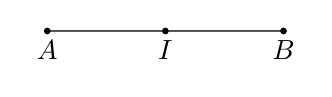
\begin{tikzpicture}[>=stealth, line join = round, line  cap = round,scale=1]
				\draw[fill] (0,0) node[below]{$ A $} circle(1pt)-- (1.5,0) node[below]{$ I $} circle(1pt) -- (3,0) node[below]{$ B $} circle(1pt);
		\end{tikzpicture}}
	}
\end{ex}



\begin{ex}%[0H1B1-3]
	Cho hình thoi $ABCD$ cạnh $a$ và $\widehat{BAD}=60^\circ $. Đẳng thức nào sau đây đúng?
	\choice
	{$\overrightarrow{BC}=\overrightarrow{DA}$}
	{$\overrightarrow{AB}=\overrightarrow{AD}$}
	{$\overrightarrow{BD}=\overrightarrow{AC}$}
	{\True $\left| \overrightarrow{BD}\right|=a$}
	\loigiai{
		Từ giả thiết suy ra tam giác $ABD$ đều cạnh $a$ nên $BD=a\Rightarrow \left| \overrightarrow{BD}\right|=a$.
	}
\end{ex}

\begin{ex}%[0H1Y1-3]
	Cho hình chữ nhật $ABCD$. Trong các đẳng thức dưới đây, đẳng thức nào đúng?
	\choice
	{$\overrightarrow{AB}=\overrightarrow{CD}$}
	{\True $\overrightarrow{AD}=\overrightarrow{BC}$}
	{$\overrightarrow{AC}=\overrightarrow{BD}$}
	{$\overrightarrow{BC}=\overrightarrow{DA}$}
	\loigiai{
		Vì $ABCD$ là hình chữ nhật nên ta có $\overrightarrow{AD}=\overrightarrow{BC}$.
	}
\end{ex}


\begin{ex}%[0H1B1-3]
	Cho tam giác $ABC$ với trung tuyến $AM$ và trọng tâm $G$. Khi đó $|\overrightarrow{GA}|$ bằng
	\choice
	{$\dfrac{1}{2}|\overrightarrow{AM}|$}
	{$\dfrac{2}{3}|\overrightarrow{GM}|$}
	{\True $2|\overrightarrow{GM}|$}
	{$-\dfrac{2}{3}|\overrightarrow{MA}|$}
	\loigiai{
		Theo tính chất đường trung tuyến $AG=\dfrac{2}{3}AM$ hay $GA=2\cdot GM$.
	}
\end{ex}

\Closesolutionfile{ans}
\Closesolutionfile{ansbook}
\indapan{10}{ans/ans-0H4-7-TN}










